
\setcounter{chapter}{11}
%----------------------------------------------------------------------------
\chapter*{11. Tétel}
%----------------------------------------------------------------------------

\textbf{Témakörök:} Grafikus, kografikus, reguláris, bináris és lineáris matroid fogalma, ezek kapcsolata (ebből bizonyítás csak a grafikus és reguláris matroidok közötti kapcsolatra), példák. Fano-matroid, példa nemlineáris matroidra. Bináris, reguláris és grafikus matroidok jellemzése tiltott minorokkal: Tutte tételei (biz. nélkül).

\noindent\hrulefill

\section*{Matroid osztályok}
\textbf{Grafikus vagy körmatroid:} $G$ gráf által indukált matroid, melyben $E=\lbrace G$ élei$\rbrace$, $F=\lbrace G$-beli erdők$\rbrace$.\\
\textbf{Kografikus:} grafikus matroid duálisa kografikus.\\
\textbf{Reguláris:} tetszőleges test felett reprezentálható.\\
\textbf{Bináris:} a kételemű (bináris) test felett reprezentálható.\\
\textbf{Lineáris:} van olyan test, ami felett reprezentálható.\\ 

\begin{figure}[h!]
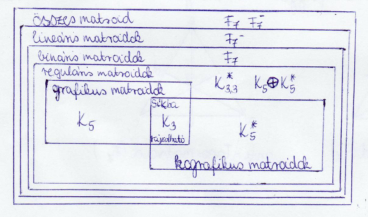
\includegraphics{matroid_osztalyok}
\centering
\end{figure}

\begin{theo}
Grafikus matroid bármely test felett reprezentálható (reguláris).
\end{theo}

\begin{theo}
Ha $M=(E,F)$ reprezentálható az $F$ test felett, akkor $M^{*}$ is. $\Rightarrow$ A kografikus matroidok is regulárisak!
\end{theo}

\section*{Karakterisztika}
Ha az $F$ testhez van olyan pozitív egész $k$, melyre teljesül, hogy az $x+x+\cdots +x$ ($k$ tagú) összeg értéke minden $x\in F$ elemre zérus, akkor a legkisebb ilyen $k$ szám a test karakterisztikája. (Minden véges testnek van karakterisztikája, ami mindig egy prím.)

\section*{Fano matroid}
Adott a hételemű halmaz: $\lbrace a,b,c,d,e,f,g \rbrace$.
\begin{itemize}
\item minden legfeljebb kételemű halmaz független
\item minden legalább négyelemű halmaz összefüggő
\item a háromeleműek közül azok függetlenek, melyeket nem köt össze vonal az ábrán
\end{itemize}

\begin{figure}[h!]
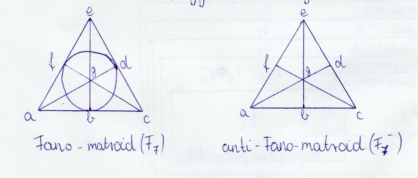
\includegraphics{fano_matroid}
\centering
\end{figure}

\section*{Tutte tételei}
\begin{itemize}
\item $M$ matroid bináris $\Leftrightarrow$ nem tartalmaz minorként $U_{4,2}$ matroidot.
\item $M$ matroid reguláris $\Leftrightarrow$ nem tartalmaz minorként $U_{4,2}$, $F_{7}$ és $F_{7}^{*}$ matroidokat.
\item $M$ matroid grafikus $\Leftrightarrow$ nem tartalmaz minorként $U_{4,2}$; $F_{7}$, $F_{7}^{*}$, $M^{*}(K_{5})$ és $M^{*}(K_{3,3})$ matroidokat.
\end{itemize}